% Preamble
\documentclass{article}

% Packages
\usepackage[legalpaper, portrati, margin=0.9in]{geometry}
\usepackage{amsmath}
\usepackage{bm}
\usepackage{amssymb}
\usepackage{gensymb}
\usepackage{mathtools}
\usepackage{xcolor}
\usepackage{caption}
\usepackage{subcaption}
\usepackage{pgfplots}
\pgfplotsset{compat=1.17}
\usepackage{tikz}
\usepackage{tkz-euclide}


% File info
\title{Geometry Notes}
\author{Eric Xia}
\date{Last Updated 21 August 2020}

% Document
\begin{document}

    \maketitle
    \tableofcontents
    \pagebreak

%%%-------------------------------------------NEW SECTION--------------------------------------%%%
    \section{Geometry Basics}

        \subsection{Common Geometrical Notations}
            \begin{center}
                \begin{tabular}{|c|c|}
                    \hline
                    \textbf{Notation} & \textbf{Definition} \\
                    \hline
                    $\angle$ & Angle \\
                    \hline
                    $\triangle$ & Triangle \\
                    \hline
                    $|F|$ & Area of Figure F \\
                    \hline
                    $\parallel$ & Parallel \\
                    \hline
                    $\perp$ & Perpendicular \\
                    \hline
                    $\sim$ & Similar to \\
                    \hline
                    $\equiv$ & Congruent to \\
                    \hline
                    $\frown \atop AB$ & Arc AB \\
                    \hline
                    $\overleftrightarrow{AB}$ & Line AB \\
                    \hline
                    $[AB],\overline{AB}$ & Line Segment AB \\
                    \hline
                    $[AB)$ & Ray AB \\
                    \hline
                    $\overrightarrow{AB}$ & Vector AB \\
                    \hline
                    $^{\circ}$ & Degrees \\
                    \hline
                    rad & Radians \\
                    \hline
                    $\pi$ & Pi Constant \\
                    \hline
                \end{tabular}
            \end{center}

        \subsection{Fundamentals of Geometry}
            A \textbf{point} has no dimensions, only position. A point is depicted by a dot. \\

            \begin{figure} [hbt!]
                \centering
                \includegraphics[scale = 0.5] {Resources/Unit1Basics/point.PNG}
                \caption*{Point P}
            \end{figure}

            \noindent A \textbf{line} is a straight one-dimensional figure with no thickness and
            extending to infinity in both directions. \textbf{Collinear points} are points existing
            on the same line. A line can be defined by two points. \textbf{Intersecting lines} are
            two lines that meet at a point. A \textbf{line segment} is a part of a line with defined
            endpoints. A line that has one defined endpoint and extends infinitely in only one
            direction is called a ray. \\

            \begin{figure} [hbt!]
                \centering
                \includegraphics[scale = 0.5] {Resources/Unit1Basics/line.PNG}
                \caption*{$\overleftrightarrow{AB}$}
            \end{figure}

            \noindent A \textbf{plane} extends infinitely in two dimensions and it has no thickness.
            A plane is defined by three non-collinear points. \\

            \begin{figure} [hbt!]
                \centering
                \includegraphics[scale = 0.3] {Resources/Unit1Basics/plane.PNG}
                \caption*{Plane ABC}
            \end{figure}

            \noindent A \textbf{space} extends infinitely in three dimensions and is a set of all
            points in three dimensions. A space can be thought of the inside of an infinitely large
            box. \\

            \begin{figure} [hbt!]
                \centering
                \includegraphics[scale = 0.3] {Resources/Unit1Basics/space.PNG}
                \caption*{A Space}
            \end{figure}

            \noindent Two figures are \textbf{congruent} if they have the same shape and size,
            whereas two figures are \textbf{similar} if they have the same shape (not necessarily
            same size). Angle and line congruency are depicted by a tick mark on the congruent
            figures. \\

            \begin{figure} [hbt!]
                \centering
                \includegraphics[scale = 0.75] {Resources/Unit1Basics/congruent.PNG}
                \caption*{$\overline{AB}\equiv\overline{CD}$}
            \end{figure}

            \noindent An \textbf{angle} is formed between two rays that share an endpoint, called
            the \textbf{vertex}. An angle is also a fraction of a circle, where the whole circle is
            $360^\circ$ or $2\pi$ radians. \textbf{Types of Angles} (Where A is an Angle): \\

            \begin{center}
                \begin{tabular}{|c|c|c|}
                    \hline
                    $A<90^\circ$ & $A<\frac{\pi}{2}$ & \textbf{Acute} Angle \\
                    \hline
                    $A=90^\circ$ & $A=\frac{\pi}{2}$ & \textbf{Right} Angle \\
                    \hline
                    $90^\circ < A < 180^\circ$ & $\frac{\pi}{2} < A < \pi$ &\textbf{Obtuse} Angle \\
                    \hline
                    $A=180^\circ$ & $\pi$ & \textbf{Straight} Angle \\
                    \hline
                \end{tabular}
            \end{center}

            \noindent Two angles are \textbf{complementary} if their measures add to $90^\circ$.
            Two angles are \textbf{supplementary} if their measures add to $180^\circ$.

            \noindent Let the endpoints of a line segment be $A(x_1, y_1)$ and $B(x_2, y_2)$. Then, \\

            \noindent \color{purple} \textbf{The Distance Formula:} \color{black}

            \begin{equation*}
                d=\sqrt{(x_2-x_1)^2+(y_2-y_1)^2}
            \end{equation*}

            \noindent \color{purple} \textbf{The Midpoint Formula:} \color{black}

            \begin{equation*}
                \text{mid}=\left(\frac{x_1+x_2}{2},\frac{y_1+y_2}{2}\right)
            \end{equation*}

        \subsection{Perpendicular and Parallel}
            Lines are \textbf{perpendicular} if they are positioned at right angles to each other.
            Perpendicular lines are depicted by a box. \\

            \begin{figure} [hbt!]
                \centering
                \includegraphics[scale = 0.6] {Resources/Unit1Basics/perpendicular.PNG}
            \end{figure}

            \noindent Lines are \textbf{parallel} if they are \textbf{equidistant}, or always the
            same distance apart, and will never meet. \\

            \begin{figure} [hbt!]
                \centering
                \includegraphics[scale = 0.4] {Resources/Unit1Basics/parallel.PNG}
                \caption*{Two parallel lines}
            \end{figure}

            \noindent \textbf{Parallel curves} are curves that are equidistant. For example, see the
            below curves \\

            \begin{figure} [hbt!]
                \centering
                \includegraphics[scale = 0.4] {Resources/Unit1Basics/parallel_curves.PNG}
            \end{figure}

            \noindent A \textbf{transversal line} is a line that crosses two other lines. When the
            two lines being crossed are parallel, \textbf{corresponding angles} are made.

            \begin{figure} [hbt!]
                \centering
                \includegraphics[scale = 0.6] {Resources/Unit1Basics/corresponding.PNG}
            \end{figure}

            \begin{center}
                \begin{tabular} {|c|c|}
                    \hline
                    $\angle A$, $\angle F$, $\angle G$, $\angle D$ & \textbf{Exterior} Angles \\
                    \hline
                    $\angle B$, $\angle E$, $\angle H$, $\angle C$ & \textbf{Interior} Angles \\
                    \hline
                    $\angle B$ and $\angle E$, $\angle H$ and $\angle C$ &\textbf{Consecutive Interior} Angles \\
                    \hline
                    $\angle A$ and $\angle G$, $\angle F$ and $\angle D$ & \textbf{Alternate Exterior} Angles \\
                    \hline
                    $\angle E$ and $\angle C$, $\angle H$ and $\angle B$ & \textbf{Alternate Interior} Angles \\
                    \hline
                    $\angle A$ and $\angle E$, $\angle C$ and $\angle G$ & \textbf{Corresponding} Angles \\
                    $\angle D$ and $\angle H$, $\angle F$ and $\angle B$ & \\
                    \hline
                \end{tabular}
            \end{center}
%
            \noindent The \textbf{perpendicular bisector} of a line is a line segment perpendicular
            to and passing through the midpoint of said line. The \textbf{angle bisector} is a line
            that splits an angle into two equal angles.

    \pagebreak
%%%----------------------------------------NEW SECTION----------------------------------------------

    \section{Triangles}

        \subsection{Triangle Basics}
            A \textbf{triangle} is a closed plane figure with three edges and three vertices.
            The interior angles of a triangle always add up to $180^\circ$. Triangles can be
            classified by their angles and sides, or both. \\

            \begin{center}
                \begin{tabular} {|c|c|c|}
                    \hline
                    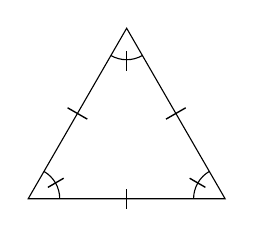
\begin{tikzpicture} [scale = 0.5, baseline=0.9cm]
                        % Draw the triangle
                        \coordinate (O) at (0,0);
                        \coordinate (A) at (5,0);
                        \coordinate (B) at (2.5,4.33);
                        \draw (O) -- (A) -- (B) -- cycle;
                        %%%
                        %Draw the line tick marks
                        \draw [line width = 0.5 pt] (2.5,-0.25) -- (2.5,0.25);
                        \draw [line width = 0.5 pt] (1.5,2.021) -- (1,2.309);
                        \draw [line width = 0.5 pt] (4,2.309) -- (3.5,2.021);
                        %%%
                        %Draw the angles
                        \tkzMarkAngle [size=0.8cm](B,A,O)
                        \tkzMarkAngle [size=0.8cm](A,O,B)
                        \tkzMarkAngle [size=0.8cm](O,B,A)
                        %%%
                        %Tick the Angles
                        \draw [line width = 0.5 pt] (2.5,3.25) -- (2.5,3.75);
                        \draw [line width = 0.5 pt] (4.5,0.288675) -- (4.1,0.52);
                        \draw [line width = 0.5 pt] (0.5,0.288) -- (0.9,0.52);
                        %%%
                    \end{tikzpicture}
                    &
                    \textbf{Equilateral} Triangle
                    & 3 Equal Sides, 3 Equal Angles \\
                    \hline

                    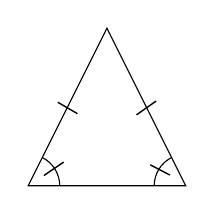
\begin{tikzpicture} [scale = 0.5]
                        %Draw the triangle
                        \coordinate (O) at (0,0);
                        \coordinate (A) at (2,4);
                        \coordinate (B) at (4,0);
                        \draw (O) -- (A) -- (B) -- cycle;
                        %%%
                        %Draw line tick marks
                        \draw [line width = 0.5 pt] (1.25,1.83) -- (0.75,2.12);
                        \draw [line width = 0.5 pt] (3.25,2.15) -- (2.75,1.8);
                        %%%
                        %Draw the angles
                        \tkzMarkAngle [size=0.8cm](B,O,A)
                        \tkzMarkAngle [size=0.8cm](A,B,O)
                        %%%
                        %Draw angle ticks
                        \draw [line width = 0.5 pt] (0.4,0.26) -- (0.9,0.6);
                        \draw [line width = 0.5 pt] (3.6,0.27) -- (3.1,0.53);
                    \end{tikzpicture}
                    &
                    \textbf{Isosceles} Triangle & 2 Equal Sides, 2 Equal Angles \\
                    \hline
                    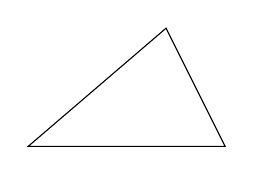
\begin{tikzpicture} [scale=0.5]
                        %Draw triangle
                        \coordinate (O) at (0,0);
                        \coordinate (A) at (3.5,3);
                        \coordinate (B) at (5,0);
                        \draw (O) -- (A) -- (B) -- cycle;
                    \end{tikzpicture}
                    & \textbf{Scalene} Triangle & No Equal Sides, No Equal Angles \\
                    \hline
                    %%%
                    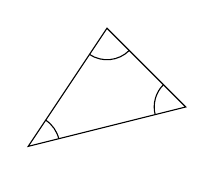
\begin{tikzpicture} [scale=0.5]
                        %Draw triangle
                        \coordinate (O) at (0,0);
                        \coordinate (A) at (2,3);
                        \coordinate (B) at (4,1);
                        \draw (O) -- (A) -- (B) -- cycle;
                        %%%
                        %Draw angles
                        \tkzMarkAngle [size=0.8cm](O,A,B)
                        \tkzMarkAngle [size=0.8cm](B,O,A)
                        \tkzMarkAngle [size=0.8cm](A,B,O)
                    \end{tikzpicture}
                    & \textbf{Acute} Triangle & All angles are less than $90^\circ$ \\
                    \hline
                    %%%
                    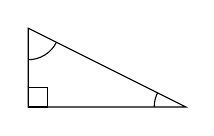
\begin{tikzpicture} [scale=0.5]
                        %Draw triangle
                        \coordinate (O) at (0,0);
                        \coordinate (A) at (0,2);
                        \coordinate (B) at (4,0);
                        \draw (O) -- (A) -- (B) -- cycle;
                        %%%
                        %Draw angles
                        \tkzMarkAngle [size=0.8cm](O,A,B)
                        \tkzMarkRightAngle [size=0.5](B,O,A)
                        \tkzMarkAngle [size=0.8cm](A,B,O)
                    \end{tikzpicture}
                    & \textbf{Right} Triangle & Has a right angle \\
                    \hline
                    %%%
                    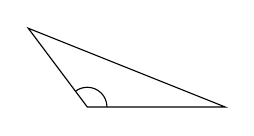
\begin{tikzpicture} [scale=0.5]
                        %Draw triangle
                        \coordinate (A) at (0,2);
                        \coordinate (B) at (1.5,0);
                        \coordinate (C) at (5,0);
                        \draw (A) -- (B) -- (C) -- cycle;
                        %%%
                        %Draw angle
                        \tkzMarkAngle [size=0.5cm](C,B,A)
                    \end{tikzpicture}
                    & \textbf{Obtuse} Triangle & Has an obtuse angle \\
                    \hline
                    %%%
                    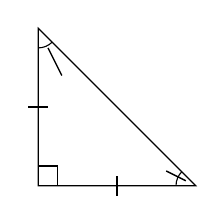
\begin{tikzpicture}[scale=0.5]
                        %Draw triangle
                        \coordinate (O) at (0,0);
                        \coordinate (A) at (4,0);
                        \coordinate (B) at (0,4);
                        \draw (O) -- (A) -- (B) -- cycle;
                        %%%
                        %Draw line ticks
                        \draw[line width=0.5 pt](2,-0.25) -- (2,0.25);
                        \draw [line width = 0.5 pt] (-0.25,2) -- (0.25,2);
                        %%%
                        %Draw angles
                        \tkzMarkAngle [size=0.5cm](O,B,A);
                        \tkzMarkAngle [size=0.5cm](B,A,O);
                        \tkzMarkRightAngle [size=0.5](B,O,A);
                        %%%
                        %Draw angle ticks
                        \draw [line width = 0.5 pt] (3.75,0.125) -- (3.25,0.375);
                        \draw [line width = 0.5 pt] (0.25,3.5) -- (0.6,2.8);
                    \end{tikzpicture}
                    & \textbf{Right Isosceles} Triangle
                    & Has a right angle and two equal angles \\
                    \hline
                \end{tabular}
            \end{center}

        \subsection{Special Triangles}
            \textbf{The $30^\circ-60^\circ-90^\circ$ Triangle}: \\

            \begin{center}
                \begin{tikzpicture} [scale=0.75]
                    %Draw triangle and label sides
                    \coordinate (O) at (0,0);
                    \coordinate (A) at (0,2);
                    \coordinate (B) at (3.4641,0);
                    \draw (A) -- (O) node[midway,left] {$a$}
                    -- (B) node[midway,below] {$a\sqrt{3}$}
                    -- (A) node[midway,right] {$2a$}
                    %%%
                    %Angles // Scale not working need to edit later
                    \tkzMarkAngle (A,B,O)
                    \tkzMarkAngle (O,A,B)
                    \tkzMarkRightAngle (A,O,B)
                \end{tikzpicture}
            \end{center}

            \noindent \textbf{The $45^\circ-45^\circ-90^\circ$ Triangle} \\

            \begin{center}
                \begin{tikzpicture} [scale=0.75]
                    %Triangle
                    \coordinate (O) at (0,0);
                    \coordinate (A) at (0,3);
                    \coordinate (B) at (3,0);
                    \draw (A) -- (O) node[midway,left] {$a$}
                    -- (B) node[midway,below] {$a$}
                    -- (A) node[midway,right] {$a\sqrt{2}$}
                    %%%
                    %Angles
                    \tkzMarkAngle (A,B,O)
                    \tkzMarkAngle (O,A,B)
                    \tkzMarkRightAngle (A,O,B)
                \end{tikzpicture}
            \end{center}

        \subsection{Triangle Formulas and Theorems}
            The \textbf{perimeter} or distance around the triangle, is given by adding up the lengths
            of the sides. Let $b$ and $h$ be the base and height of a triangle, respectively. Then, \\

            \noindent \color{purple} \textbf{Area of a Triangle:} \color{black}

            \begin{equation*}
                A=\frac{bh}{2}
            \end{equation*}

            \begin{center}
                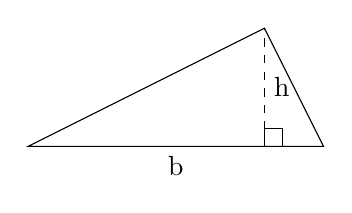
\begin{tikzpicture} [scale = 0.75]
                    %Draw triangle and base
                    \coordinate (O) at (0,0);
                    \coordinate (A) at (4,2);
                    \coordinate (B) at (5,0);
                    \coordinate (C) at (4,0);
                    \draw (O) -- node [midway, below] {b} (B) -- (A) -- cycle;
                    %%%
                    %Draw height
                    \draw [dashed] (4,0) --(4,2) node [midway, right] {h};
                    %%%
                    %Draw right angle
                    \tkzMarkRightAngle [size=0.3](B,C,A)
                \end{tikzpicture}
            \end{center}

            \noindent \color{purple} \textbf{Heron's Formula} \color{black} states that if $a,b,$ and
            $c$ are the sides of a triangle and $s$ is the triangle's \textbf{semiperimeter}, or half
            the perimeter, then the area of a triangle is given by \\

            \begin{equation*}
                A = \sqrt{s(s-a)(s-b)(s-c}
            \end{equation*}

            \noindent \color{purple} \textbf{The Pythagorean Theorem:} \color{black} for any right
            triangle with sides $a,b,c$,$c$ being the hypotenuse, \\

            \begin{equation*}
                a^2 + b^2 = c^2
            \end{equation*}

            \noindent $3,4,5$ and $5,12,13$ are some special Pythagorean numbers, called
            \textbf{Pythagorean Triples} due to their properties as integers. \\

            \noindent The \color{purple} \textbf{Triangle Inequality Theorem} \color{black} states
            that if a figure is a triangle then the sum of the lengths of any two sides is greater
            than the length of the third side. The contrapositive of this theorem also holds.

            \noindent The angle between two intersecting lines, where $m_1$ and $m_2$ are the slopes
            of the lines, is given by \\

            \begin{equation*}
                \theta = \arctan{\left|\frac{m_2-m_1}{1+m_2m_1}\right|}
            \end{equation*}

        \subsection{Construction with Triangles}
            A \textbf{median} of a triangle is a segment from a vertex to the midpoint of the opposite
            side. The \textbf{centroid} is the point at which the three medians of a triangle intersect
            and is also the centre of mass of the triangle. The \color{purple} \textbf{Centroid Theorem}
            \color{black} states that the centroid is located $\frac{2}{3}$ of the distance from each
            vertex to the midpoint of the opposite side. \\

            \begin{figure} [hbt!]
                \centering
                \includegraphics[scale = 0.075] {Resources/Unit2Triangles/centroid.PNG}
                \caption*{Medians and Centroid of a Triangle}
            \end{figure}

            \noindent An \textbf{altitude} of a triangle is a segment from a vertex constructed
            perpendicular to the opposite side. The \textbf{orthocenter} is the point at which the
            three altitudes of a triangle meet.

            \begin{figure} [hbt!]
                \centering
                \includegraphics[scale = 0.08] {Resources/Unit2Triangles/orthocenter.PNG}
                \caption*{Altitudes and Orthocenter of a Triangle}
            \end{figure}

            \noindent The \textbf{incircle} is also known as the inscribed circle. The center of
            this circle is called the \textbf{incenter} and is equidistant from all sides of the
            triangle. \\

            \begin{figure} [hbt!]
                \centering
                \includegraphics[scale = 0.75] {Resources/Unit2Triangles/incircle.jpg}
                \caption*{Incircle}
            \end{figure}

            \noindent The \textbf{circumcircle} is also known as the circumscribed circle. \\
            \begin{figure} [hbt!]
                \centering
                \includegraphics[scale = 0.75] {Resources/Unit2Triangles/circumcircle.PNG}
                \caption*{Circumcircle}
            \end{figure}

        \subsection{Congruent and Similar Triangles}
            \color{purple} \textbf{The 5 Congruency Postulates:} \color{black} \\

            \noindent \color{purple}\textbf{1. SSS (Side, Side, Side)} \color{black}\\
            \noindent If two triangles share three equal sides then the two triangles are congruent. \\

            \noindent \color{purple}\textbf{2. SAS (Side, Angle, Side)}\color{black} \\
            \noindent If two triangles share two equal sides and an equal angle between said sides
            then the two triangles are congruent. \\

            \noindent \color{purple}\textbf{3. ASA (Angle, Side, Angle)}\color{black} \\
            \noindent If two triangles share two equal angles and an equal side between said angles
            then the two triangles are congruent. \\

            \noindent \color{purple}\textbf{4. AAS (Angle, Angle, Side)}\color{black} \\
            \noindent If two triangles share two equal angles and one equal side all consecutively,
            then the two triangles are congruent. \\

            \noindent \color{purple}\textbf{5. HL (Hypotenuse, Leg)}\color{black} \\
            \noindent If two triangles share the same hypotenuse and any one of the other legs,
            then the two triangles are congruent. \\

            \noindent Similar triangles have proportional corresponding sides. For example, \\

            \begin{figure} [hbt!]
                \centering
                \includegraphics[scale = 0.6] {Resources/Unit2Triangles/sim1.PNG}
                \caption*{$\frac{AD}{DB}=\frac{EC}{BE}$}
            \end{figure}

            \noindent and \\

            \begin{figure} [hbt!]
                \centering
                \includegraphics[scale = 0.8] {Resources/Unit2Triangles/sim2.PNG}
                \caption*{$\frac{AD}{DC}=\frac{AB}{BC}$}
            \end{figure}

        \subsection{The Laws of Sine and Cosine}
            For any angles $A$,$B$, and $C$, the following definitions hold true.

            \begin{center}
                \begin{tabular}{ccc}
                    $\sin A = \frac{a}{c}$
                    & $\cos A = \frac{b}{c}$
                    & $\tan A = \frac{a}{b}$ \\
                    $\csc A = \frac{c}{a}$
                    & $\sec A = \frac{c}{b}$
                    & $\cot A = \frac{b}{a}$\\\\
                    $\sin B = \frac{b}{c}$
                    & $\cos B = \frac{a}{c}$
                    & $\tan B = \frac{b}{a}$
                \end{tabular}
            \end{center}

            \begin{figure} [h]
                \centering
                \includegraphics [scale=0.4] {Resources/Unit2Triangles/Trig.fig1.png}
            \end{figure}

            \noindent From the figure, it is easy to tell that $\sin A$ and $\csc A$, $\cos A$ and
            $\sec A$, and $\tan A$ and $\cot A$ are reciprocal functions. Hence, it is usually easier
            to just work with $\sin A$, $\cos A$, and $\tan A$ Additionally,

            \begin{center}
                \begin{tabular}{ccc}
                    $\frac{\sin A}{\cos A}=\tan A$
                    & and &
                    $\frac{\cos A}{\sin A}=\cot A$
                \end{tabular}
            \end{center}

            \noindent \color{purple} \textbf{The Law of Sines}:  \color{black}

            \begin{equation*}
                \frac{a}{\sin{A}} = \frac{b}{\sin{B}} = \frac{c}{\sin{C}}
            \end{equation*} \\

            \noindent and

            \begin{equation*}
                \frac{\sin{A}}{a} = \frac{\sin{B}}{b} = \frac{\sin{C}}{c}
            \end{equation*}

            \begin{center}
                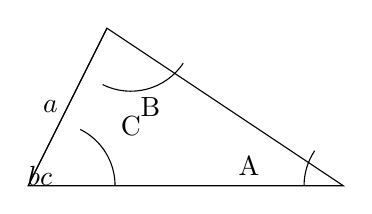
\begin{tikzpicture} [scale=1]
                    %Draw triangle
                    \coordinate (O) at (0,0);
                    \coordinate (A) at (1,2);
                    \coordinate (B) at (4,0);
                    \draw (O) -- (A) -- (B) -- cycle;
                    %Side markings
                    \draw (A) -- (O) node[midway,left] {$a$};
                    -- (B) node[midway,below] {$b$};
                    -- (A) node[midway,right] {$c$};
                    %Angles
                    \tkzMarkAngle [size=0.8cm](O,A,B);
                    \tkzMarkAngle [size=0.8cm](B,O,A);
                    \tkzMarkAngle [size=0.8cm](A,B,O);
                    %Angle markings \\Need to fix instead of brute forcing anchor points
                    \draw (1,1) node[below] {C};
                    \draw (1,1) node[below, right] {B};
                    \draw (2.5,0) node[left, above] {A};
                \end{tikzpicture}
            \end{center}

            \noindent \color{purple} \textbf{The Law of Cosines:} \color{black} \\

            \begin{equation*}
                a^2 = b^2 + c^2 -2bc \cos{A}
            \end{equation*}

            \noindent and

            \begin{equation*}
                \cos{A}=\frac{b^2+c^2-a^2}{2bc}
            \end{equation*}

        \subsection{Ceva's Theorem}
            A \textbf{cevian} is a line that intersects both a triangle's vertex and the side
            opposite to said vertex. Medians and angle bisectors are special cases of cevians.
            \color{purple} \textbf{Ceva's Theorem} \color{black} is a criterion for the concurrence
            of cevians in a triangle. \textbf{Concurrence} means that several lines or curves
            intersect at a certain point. \\

            \noindent It states that if $ABC$ is a triangle and $D,E,F$ are all points on
            $\overline{BC},\overline{CA},\overline{AB}$, respectively, then $\overline{AD},
            \overline{BE},\overline{CF}$ are concurrent if and only if \\

            \begin{equation*}
                \frac{BD}{DC}\cdot\frac{CE}{EA}\cdot\frac{AF}{FB}=1
            \end{equation*}

            \noindent Since the reciprocal of 1 is 1, the reciprocals of the ratios also have a
            product of 1. \\

            \begin{figure} [hbt!]
                \centering
                \includegraphics[scale=0.75]{Resources/Unit2Triangles/ceva.PNG}
            \end{figure}

        \pagebreak
        \subsection{Menelaus' Theorem}
            \color{purple} \textbf{Menelaus' Theorem} \color{black} describes the collinearity of
            points on each of the three sides of a triangle. It states that if $\overline{PQ}$
            intersects $\overline{AB}$ on $\triangle ABC$ where $P$ is on $\overline{BC}$, $Q$ is
            the extension of $\overline{AC}$, and $R$ is on the intersection of $\overline{PQ}$ and
            $\overline{AB}$, then \\

            \begin{equation*}
                \frac{PB}{CP}\cdot\frac{QC}{QA}\cdot\frac{AR}{RB}=1
            \end{equation*}

            \begin{figure} [hbt!]
                \centering
                \includegraphics[scale=0.75]{Resources/Unit2Triangles/menelaus.PNG}
            \end{figure}

    \pagebreak
%%%------------------------------------------NEW SECTION-------------------------------------------

    \section{Polygons}

        \subsection{Polygon Basics}
            \textbf{Polygons} are closed 2D figures composed of straight lines. By this definition,
            any figure that has a curve or is open is not a polygon. A \textbf{regular polygon} has
            all angles and sides equal. An \textbf{irregular polgyon} is any polygon that is not
            regular. A \textbf{convex polygon} has no inwardly-pointing (greater than $180^\circ$)
            angles. A \textbf{concave polygon} is any polygon with at least one internal angle
            greater than $180^\circ$. A \textbf{simple polygon} does not self-intersect, whereas a
            \textbf{complex polygon} self-intersects. \\

            \noindent \color{purple} \textbf{Common Regular Polygons:} \color{black} \\

            \begin{center}
                \begin{tabular}{|c|c|}
                    \hline
                    \textbf{Name} & \textbf{Sides} \\
                    \hline
                    Triangle (Trigon) & 3 \\
                    \hline
                    Quadrilateral (Tetragon) & 4 \\
                    \hline
                    Pentagon & 5 \\
                    \hline
                    Hexagon & 6 \\
                    \hline
                    Heptagon (Septagon) & 7 \\
                    \hline
                    Octagon & 8 \\
                    \hline
                    Nonagon (Enneagon) & 9 \\
                    \hline
                    Decagon & 10 \\
                    \hline
                    n-gon & n \\
                    \hline
                \end{tabular}
            \end{center}

            \noindent \color{purple} \textbf{Naming Prefixes and Suffixes: } \color{black} \\

            \begin{center}
                \begin{tabular}{|c|c|}
                    \hline
                    \textbf{Sides} & \textbf{Prefixes/Suffixes} \\
                    \hline
                    20 & Icosi- \\
                    \hline
                    30 & Triaconta- \\
                    \hline
                    40 & Tetraconta- \\
                    \hline
                    50 & Pentaconta- \\
                    \hline
                    60 & Hexaconta- \\
                    \hline
                    70 & Heptaconta- \\
                    \hline
                    80 & Octaconta- \\
                    \hline
                    90 & Enneaconta-/Nonaconta- \\
                    \hline
                    100 & Hecta- \\
                    \hline
                    +1 & -henagon \\
                    \hline
                    +2 & -digon \\
                    \hline
                    +3 & -trigon \\
                    \hline
                    +4 & -tetragon \\
                    \hline
                    +5 & -pentagon \\
                    \hline
                    +6 & -hexagon \\
                    \hline
                    +7 & -heptagon \\
                    \hline
                    +8 & -octagon \\
                    \hline
                    +9 & -nonagon/-enneagon \\
                    \hline
                \end{tabular}
            \end{center}

            \noindent Given a convex polygon with $n$ sides, we can find the sum of the interior
            angles, $S$, such that \\

            \begin{equation*}
                S = 180(n-2)
            \end{equation*}

            \noindent The sum of all the exterior angles for a convex polygon always add to
            $360^\circ$.

        \subsection{Quadrilaterals}
            For quadrilaterals, the sum of all interior angles always add to $360^\circ$.

            \begin{figure} [hbt!]
                \centering
                \caption*{\color{purple}Types of Quadrilaterals:\color{black}}
                \includegraphics[scale = 0.8] {Resources/Unit3Polygons/quad.PNG}
            \end{figure}

            \noindent The diagonals of a rhombus bisect each other. Therefore, if a parallelogram
            has diagonals that bisect each other, then the parallelogram is a rhombus. For kites,
            the angles where the two pairs meet are equal, the diagonals meet at right angles, and
            one of the diagonals bisects the other. \\

            \noindent The square is the only regular quadrilaterals and all other quadrilaterals are
            irregular. \\

            \pagebreak
            \noindent \color{purple} \textbf{Quadrilateral Area Formulas:} \color{black} \\

            \begin{center}
                \begin{tabular} {|c|c|}
                    \hline
                    $A=s^2$, $s$ = side & Square \\
                    \hline
                    $A=bh$, $b$ = base, $h$ = height & Rectangle \\
                    \hline
                    $A=\frac{pq}{2}$, $p$ and $q$ are diagonals & Rhombus \\
                    \hline
                    $A=bh$, $b$ = base, $h$ = height & Parallelogram \\
                    \hline
                    $A=h(\frac{b_1+b_2}{2})$, $b_1$ and $b_2$ are bases, $h$ = height & Trapezoid \\
                    \hline
                    $A=\frac{pq}{2}$, $p$ and $q$ are diagonals & Kite \\
                    \hline
                \end{tabular}
            \end{center}

    \pagebreak

%%%-------------------------------------------NEW SECTION--------------------------------------%%%
    \section{Circles}

        \subsection{Circle Basics}
            A \textbf{circle} is a 2D figure composed of all the points that are a given distance
            (\textbf{radius}) away from a centre. The \textbf{diameter} of a circle is the distance
            from one side of the circle to the other, passing through the centre of the circle.
            It is double the length of the radius. The \textbf{circumference} of a circle is the
            distance around the circle. \\

            \noindent When $d$ is the diameter of a circle, the circumference of said circle, $C$,
            is given by \\

            \begin{equation*}
                C = \pi d
            \end{equation*}

            \noindent The area of any circle is given by \\

            \begin{equation*}
                A=\pi r^2
            \end{equation*}

            \noindent A circle has about 80\% of the area of an equal-width square. \\

            \noindent A \textbf{tangent} is a line that intersects the edge of a circle only once
            and is perpendicular at the intersection point. A line that intersects a circle twice
            is called a \textbf{secant}. A \textbf{chord} is a line segment travelling between any
            two points on a circle's circumference. A \textbf{diameter} is also a chord that passes
            through the centre of the circle. An \textbf{arc} is any section of the circumference.
            A \textbf{sector} is any part of a circle enclosed by two radii and their intercepted
            arc. A \textbf{segment} is any slice on a circle made by a chord. A quarter of a circle
            is a \textbf{quadrant} and half a circle is a \textbf{semicircle}. \\

            \begin{figure} [hbt!]
                \centering
                \includegraphics[scale = 0.8] {Resources/Unit4Circles/lines.PNG}
                \includegraphics[scale = 0.8] {Resources/Unit4Circles/slices.PNG}
            \end{figure}

            \noindent The arc of a circle, $s$, where $\theta$ is the intercepted angle between the
            two radii composing the arc \textit{measured in RADIANS}, is given by \\

            \begin{equation*}
                s=r\theta
            \end{equation*}

            \noindent The area of a sector, where $\theta$ is the intercepted angle between the two
            radii composing the sector \textit{measured in RADIANS}, is given by \\

            \begin{equation*}
                A=\frac{1}{2} r^2 \theta
            \end{equation*}

            \noindent \color{purple} \textbf{The 7 Common Circle Theorems:} \color{black} \\

            \noindent \color{purple} \textbf{1. Angle at the Centre Theorem} \color{black} \\

            \begin{figure} [hbt!]
                \centering
                \includegraphics[scale=0.6]{Resources/Unit4Circles/circle1.PNG}
            \end{figure}

            \noindent The angle formed at the centre of a circle by lines originating from any two
            points on the circle's circumference is double the angle formed on the circumference of
            the circle by lines originating from the same points. \\

            \pagebreak
            \noindent \color{purple} \textbf{2. Angle in a Semicircle Theorem} \color{black} \\
            \begin{figure} [hbt!]
                \centering
                \includegraphics[scale=0.75]{Resources/Unit4Circles/circle2.PNG}
            \end{figure}

            \noindent An angle formed by constructing lines from the ends of the diameter of a circle
            to its circumference form a right angle. \\

            \noindent \color{purple} \textbf{3. Angles in the Same Segment} \color{black} \\

            \begin{figure} [hbt!]
                \centering
                \includegraphics[scale=0.7]{Resources/Unit4Circles/circle3.PNG}
            \end{figure}

            \noindent Angles formed from two points on the circumference are equal to other angles
            in the same arc formed from said points. \\

            \noindent \color{purple} \textbf{4. Cyclic Quadrilaterals} \color{black} \\

            \begin{figure} [hbt!]
                \centering
                \includegraphics[scale=0.6]{Resources/Unit4Circles/circle4.PNG}
            \end{figure}

            \noindent The opposite angles of a cyclic quadrilateral are equal. \\

            \noindent \color{purple}\textbf{5. Radius to a Tangent} \color{black} \\

            \begin{figure} [hbt!]
                \centering
                \includegraphics[scale=0.75]{Resources/Unit4Circles/circle5.PNG}
            \end{figure}

            \noindent The radius and tangent that intercept any point on a circle's circumference
            form a right angle. \\

            \pagebreak
            \noindent \color{purple} \textbf{6. Tangents from a Point to a Circle} \color{black} \\

            \begin{figure} [hbt!]
                \centering
                \includegraphics[scale=0.75]{Resources/Unit4Circles/circle6.PNG}
            \end{figure}

            \noindent When two tangents are constructed on the same circle, the distance between
            their point of intersection with the circle and point of intersection with each other
            is the same. Furthermore, when a line from the intersection point of the two tangents
            to the centre of the circle is constructed, the angles formed between said line and
            either tangent are equal. \\

            \noindent \color{purple} \textbf{7. Alternate Segment Theorem} \color{black} \\

            \begin{figure} [hbt!]
                \centering
                \includegraphics[scale=0.75]{Resources/Unit4Circles/circle7.PNG}
            \end{figure}

            \noindent The alternate angles inside two segments constructed within a circle are equal.

        \subsection{Power of a Point Theorem}
            The \color{purple} \textbf{Power of a Point Theorem} \color{black} is a relationship
            holding between the lengths of the line segments formed when two lines intersect a circle
            and each other. There are three possibilities for which this theorem holds: \\

            \noindent 1. The two lines are chords of the circle and intersect inside the circle.
            In this case, we have $AE\cdot CE = BE\cdot DE$. \\

            \begin{figure} [hbt!]
                \centering
                \includegraphics[scale=0.75]{Resources/Unit4Circles/power1.PNG}
            \end{figure}

            \noindent 2. One line is a tangent and the other is a secant. In this case, we have
            $AB^2=BC\cdot BD$. \\

            \begin{figure} [hbt!]
                \centering
                \includegraphics[scale=0.75]{Resources/Unit4Circles/power2.PNG}
            \end{figure}

            \pagebreak
            \noindent 3. Both lines are secants and intersect outside the circle. In this case,
            $CB\cdot CA = CD\cdot CE$. \\

            \begin{figure} [hbt!]
                \centering
                \includegraphics[scale=0.75]{Resources/Unit4Circles/power3.PNG}
            \end{figure}

    \pagebreak
%%%-------------------------------------------NEW SECTION--------------------------------------%%%

    \section{Transformations}
        \color{purple} \textbf{The 4 Main Geometrical Transformations:} \color{black} \\

        \begin{figure} [hbt!]
            \centering
            \begin{subfigure}[b]{.45\linewidth}
                \includegraphics[scale=0.5]{Resources/Unit5Transformations/rotation.PNG}
                \caption*{Rotation}
            \end{subfigure}
            \begin{subfigure}[b]{.45\linewidth}
                \includegraphics[scale=0.5]{Resources/Unit5Transformations/reflection.PNG}
                \caption*{Reflection}
            \end{subfigure}
            \begin{subfigure}[b]{.45\linewidth}
                \includegraphics[scale=0.5]{Resources/Unit5Transformations/translation.PNG}
                \caption*{Translation}
            \end{subfigure}
            \begin{subfigure}[b]{.45\linewidth}
                \includegraphics[scale=0.5]{Resources/Unit5Transformations/homothety.PNG}
                \caption*{Homothety}
            \end{subfigure}
        \end{figure}

        \noindent When homothety is used to transform a figure, the figure and its result are
        similar. If a figure is transformed by any method besides homothety, the figure and its
        result are congruent.

    \pagebreak
%%%-------------------------------------------NEW SECTION--------------------------------------%%%

    \section{Solids}

        \subsection{Basics of Solids}
            A \textbf{solid} is a 3D figure. A \textbf{face} of a solid is a flat surface. A
            \textbf{edge} of a solid is where 2 or more faces meet. A \textbf{vertex} is where 2 or
            more straight edges meet. \\

        \subsection{Polyhedra}
            \noindent A \textbf{polyhedron} is a solid composed only of flat faces and each face is
            a polygon. Common polyhedra include the platonic solids, prisms, and pyramids. \\

            \noindent The \textbf{Platonic Solids} are solids where each face is the same regular
            polygon and the same number of polygons meet at each vertex. In $\mathbb{R}^3$ there are
            5 Platonic Solids, of which each was theorized by Plato to represent the five elements:
            earth, air, fire, water, and the universe. \\

            \begin{figure} [hbt!]
                \centering
                \begin{subfigure}[b]{.45\linewidth}
                    \includegraphics[scale=0.25]{Resources/Unit6Solids/tetrahedron.png}
                    \caption*{Tetrahedron}
                \end{subfigure}
                \begin{subfigure}[b]{.45\linewidth}
                    \includegraphics[scale=0.5]{Resources/Unit6Solids/cube.PNG}
                    \caption*{Cube}
                \end{subfigure}
                \begin{subfigure}[b]{.45\linewidth}
                    \includegraphics[scale=1]{Resources/Unit6Solids/octahedron.PNG}
                    \caption*{Octahedron}
                \end{subfigure}
                \begin{subfigure}[b]{.45\linewidth}
                    \includegraphics[scale=0.25]{Resources/Unit6Solids/dodecahedron.PNG}
                    \caption*{Dodecahedron}
                \end{subfigure}
                \begin{subfigure}[b]{.45\linewidth}
                    \includegraphics[scale=0.4]{Resources/Unit6Solids/icosahedron.PNG}
                    \caption*{Icosahedron}
                \end{subfigure}
            \end{figure}

            \noindent A \textbf{prism} is a polyhedron with identical ends and the same cross-section
            along its length. Let $B$ and $h$ represent the base and height of a prism. Then  \\

            \noindent \color{purple} \textbf{Volume of a Prism:} \color{black}
            \begin{equation*}
                V = Bh
            \end{equation*}

            \noindent A \textbf{pyramid} is any polyhedron where there is a polygon base and all
            other faces are triangles. The other faces all connect the base to the \textbf{apex}. \\

            \noindent \color{purple} \textbf{Volume of a Pyramid:} \color{black} \\
            \begin{equation*}
                V = \frac{Bh}{3}
            \end{equation*}

        \subsection{Non-Polyhedrons}
            \textbf{Nonpolyhedrons} have curved surfaces. Common non-polyhedrons include spheres,
            cylinders, cones, and tori. \\

            \noindent \textbf{Spheres} are 3D figures where all points on the surface are the same
            distance from a center. Spheres are perfectly symmetrical, have no edges nor vertices,
            and only have one surface. Of all the solids, spheres have the greatest volume to surface
            area ratio. A \textbf{hemisphere} is half of a sphere. \\

            \pagebreak
            \noindent \color{purple} \textbf{Surface Area of a Sphere:} \color{black} \\

            \begin{equation*}
                A = 4\pi r^2
            \end{equation*}

            \noindent \color{purple} \textbf{Volume of a Sphere:} \color{black} \\

            \begin{equation*}
                \frac{4}{3}\pi r^3
            \end{equation*}

            \noindent A \textbf{cylinder} is a non-polyhedron with straight parallel sides and an
            ellipse cross-section. A \textbf{Right Cylinder} is a cylinder with its two bases
            directly aligned on top of each other. An \textbf{Oblique Cylinder} is any cylinder
            that is not right.

            \begin{figure} [hbt!]
                \centering
                \includegraphics[scale=0.5]{Resources/Unit6Solids/cylinders.png}
                \caption*{Right and Oblique Cylinders}
            \end{figure}

            \noindent \color{purple} \textbf{Surface Area of a Cylinder}: \color{black}

            \begin{equation*}
                A=2\pi rh+2\pi r^2
            \end{equation*}

            \noindent \color{purple} \textbf{Volume of a Cylinder:} \color{black}

            \begin{equation*}
                V=\pi r^2 h
            \end{equation*}

            \noindent A \textbf{cone} is a non-polyhedron that tapers smoothly from a flat base
            to an \textbf{apex}. It can be formed by rotating a triangle $360^\circ$ in along
            the dependent axis. When the apex of a cone is aligned with the centre of the base,
            it is a \textbf{right cone}. Otherwise, the cone is \textbf{oblique}. \\

            \begin{figure} [hbt!]
                \centering
                \includegraphics[scale=0.5]{Resources/Unit6Solids/cones.jpg}
                \caption*{Right and Oblique Cylinders}
            \end{figure}

            \noindent \color{purple} \textbf{Surface Area of a Right Cone}: \color{black} \\

            \begin{equation*}
                A=\pi r(r+\sqrt{h^2+r^2})
            \end{equation*}

            \noindent \color{purple} \textbf{Volume of a Cone}: \color{black} \\

            \begin{equation*}
                V = \frac{\pi r^3h}{3}
            \end{equation*}

            \noindent The \textbf{torus} is a solid of revolution generated by revolving a
            circle in $\mathbb{R}^3$ about an axis coplanar with the circle. Its shape resembles
            that of a donut. For tori, $r$ is the smaller radius of the circle cross-section and
            $R$ is the larger radius around which the circle is swept, such that \\

            \begin{figure} [hbt!]
                \centering
                \includegraphics[scale=0.5]{Resources/Unit6Solids/torus.png}
            \end{figure}

            \noindent \color{purple} \textbf{Surface Area of a Torus}: \color{black} \\

            \begin{equation*}
                A = 4 {\pi}^2 Rr
            \end{equation*}

            \noindent \color{purple} \textbf{Volume of a Torus}: \color{black} \\

            \begin{equation*}
                V = 2 {\pi}^2 Rr^2
            \end{equation*}


\end{document}